\documentclass[12pt, a4paper]{article}

% ── PAQUETES ─────────────────────────────────────────────────
% Los paquetes amplían las capacidades de LaTeX.
% Se cargan en el "preámbulo" (antes de \begin{document}).

\usepackage[utf8]{inputenc}       % Permite tildes y ñ
\usepackage[spanish]{babel}       % Idioma español (guiones, fechas, etc.)
\usepackage{geometry}             % Control de márgenes
\usepackage{graphicx}             % Para insertar imágenes
\usepackage{setspace}             % Control de interlineado
\usepackage{hyperref}             % Links clicables (índice, URLs)
\usepackage{xcolor}               % Colores personalizados
\usepackage{listings}
\usepackage{tcolorbox}
\usepackage{amsmath}
\usepackage{float}
\usepackage{booktabs}
\tcbuselibrary{listings, skins}

\newtcblisting{terminal}{
    colback   = black,           % fondo negro
    colframe  = gray!50,         % borde gris
    coltitle  = black,           % título en blanco
    coltext   = green!70!white,  % texto verde (estilo terminal clásica)
    title     = Terminal,
    fonttitle = \bfseries\small,
    listing only,
    listing options = {
        basicstyle = \ttfamily\small\color{green!70!white},
        breaklines = true,
    }
}

\lstset{
    basicstyle    = \ttfamily\small,   % fuente monoespaciada
    keywordstyle  = \color{blue},      % palabras clave en azul
    commentstyle  = \color{gray},      % comentarios en gris
    stringstyle   = \color{orange},    % strings en naranja
    numbers       = left,              % números de línea a la izquierda
    frame         = single,            % recuadro alrededor del bloque
    breaklines    = true,              % corta líneas largas automáticamente
}

\newcommand{\tema}{Laboratorio Nº1: Verilog}
\newcommand{\titulotrabajo}{Informe}
\newcommand{\autor}{Alfici, Facundo Ezequiel}
\newcommand{\documento}{44012327}
\newcommand{\curso}{PROCOM}
\newcommand{\fundacion}{Fundación Fulgor}
\newcommand{\fecha}{\today}

% ── INICIO DEL DOCUMENTO ─────────────────────────────────────
% Todo lo visible va DENTRO de este entorno
\begin{document}

% Quitamos la numeración en la carátula
\thispagestyle{empty}

% ── CARÁTULA ─────────────────────────────────────────────────
\begin{center}   % Entorno para centrar contenido

    % --- Encabezado institucional ---
    {\Large \textbf{\fundacion}}\\[0.3cm]      % \\ fuerza un salto de línea                 % [0.2cm] = espacio extra después
    {\large \curso}

    \vspace{1.5cm}   % Espacio vertical de 1.5 cm

    % --- Logo (opcional) ---
    % Descomenta las 2 líneas siguientes si tenés un logo guardado
    % \includegraphics[width=0.25\textwidth]{logo.png}
    % \vspace{1cm}

    \hrule height 1pt   % Línea horizontal
    \vspace{0.4cm}

    % --- Título del trabajo ---
    {\LARGE \textbf{\titulotrabajo}}\\[0.3cm]
    {\large \tema}

    \vspace{0.4cm}
    \hrule height 1pt

    \vspace{2.5cm}

    % --- Datos del alumno ---
    % Tabla simple de 2 columnas: etiqueta y valor
    \begin{tabular}{r l}   % r = columna alineada a la derecha, l = izquierda
        \textbf{Autor:}   & \autor\\[0.2cm]
        \textbf{Documento:}  & \documento\\[0.2cm]
        \textbf{Docentes:} &  Ariel Pola, Santiago Garaventta Pascual y Agustín Pesce\\
    \end{tabular}

    \vspace{3cm}

    % --- Fecha ---
    {\large \fecha}

\end{center}

% Salto de página → el informe real comienza en la siguiente hoja
\newpage

% ── EJEMPLO DE PRIMERA SECCIÓN (para no dejar el doc vacío) ──
\tableofcontents   % Genera el índice automáticamente
\newpage


%Cuerpo del informe

\section{Introducción}
En este laboratorio se implementó un código de \textbf{Verilog} encargado de realizar un desplazamiento por medio de un shift register. Éste desplazamiento se observaba de forma visual sobre la placa,
donde la idea fue encender cierto LED cada vez que el desplazamiento se presentaba.

El desplazamiento se realizó de forma circular, utilizando una variable de 4 bits llamada \textbf{i\_sw}, que representaba los switches de la placa física. Con esta variable, se manejó ciertos parámetros del
desplazamiento. Se listan a continuación los parámetros a controlar:
    \begin{itemize}
        \item \textbf{Enable:} Mediante el i\_sw[0], se habilita o deshabilita el contador. En estado cero '0' se detiene el funcionamiento, mientras que en estado uno
        '1' se activa el desplazamiento. Es importante destacar que en caso de deshabilitar el contador, éste mantendrá su estado actual, de igual manera que ocurre con el shift register.
        \item \textbf{Límite de conteo:} Utilizando los bits i\_sw[2:1], se permite realizar una selección del límite superior de conteo. Contando con 4 valores posibles.
        \item \textbf{Color del led:} El bit i\_sw[3] se encarga de seleccionar el color del LED a encender durante el desplazamiento.
    \end{itemize}
\newpage

\section{Desarrollo}
El código se desarrolló utilizando el software \textbf{Vivado 2024.2}, donde el proceso se dividió en 2 partes;
\begin{enumerate}
    \item \texttt{Apartado de Código:} Creación de jerarquía, escritura del código y simulación por medio de un testbench.
    \item \texttt{Apartado de Implementación}Adición de constraint, síntesis, implementación, bitstream y conexión por hardware.
\end{enumerate}
Estas partes se detallarán a continuación, comenzando con el primer proyecto realizado.
\subsection{Apartado de Código}
En este apartado, se realizó la escritura del código, mediante lo visto y propuesto durante las clases. Para ello, se utilizó una estructura jerárquica donde se dividió el código en submódulos.
Dentro de estos submódulos, se encuentran el módulo del contador, denominado \texttt{count.v}, el módulo del shift register, denominado \texttt{shiftreg.v} y el módulo principal que contiene a ambos, llamado
\texttt{topModule.v}.

La jerarquía se puede ver en la siguiente imagen.
\begin{figure}[H]
    \centering
    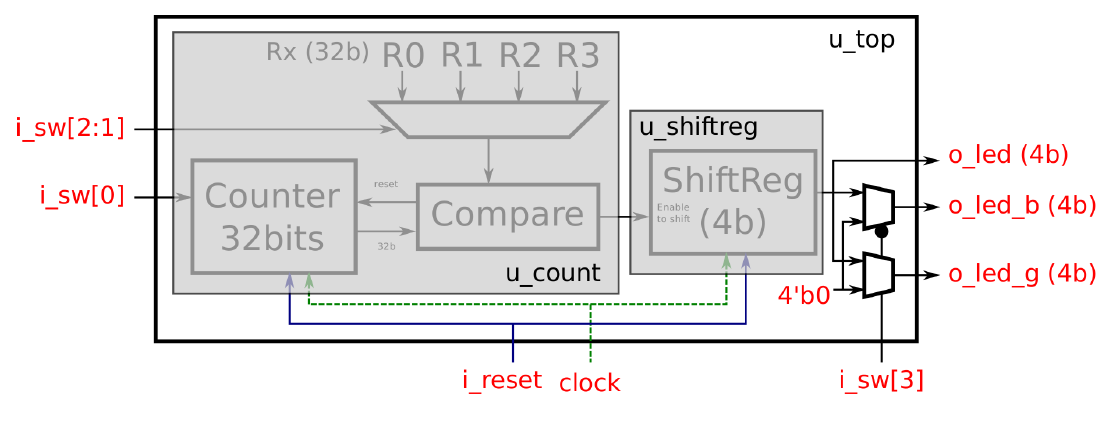
\includegraphics[width=0.9\textwidth]{imagenes_lab01/diagrama_jerarquia.png}
    \caption{Diagrama jerárquico del proyecto.}
    \label{fig:jerarquia}
\end{figure}
Con los códigos terminados, se procedió a realizar la simulación por medio del testbench generado en clase, llamado \texttt{tb\_topModule.v}. El código generará estímulos para cada uno de las variaciones
posibles de los parámetros existentes. Sabiendo esto, en la siguiente imagen se muestra el comportamiento del diseño, ignorando los IP cores VIO e ILA en primera instancia.
\begin{figure}[H]
    \centering
    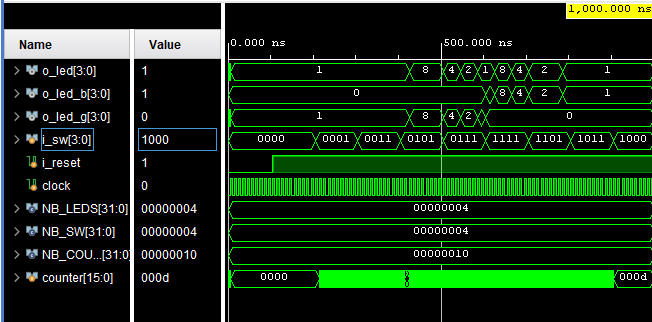
\includegraphics[width=0.9\textwidth]{imagenes_lab01/tb_top.png}
    \caption{Testbench del topModule.}
    \label{fig:tb_top}
\end{figure}
El testbench tiene una linea de flujo de cambios, donde de manera principal se generan cambios en el parámetro i\_sw para poder ver el cambio en los valores del contador.

\begin{center}
i\_sw = 0000 $\rightarrow$ i\_sw = 0001 $\rightarrow$ i\_sw = 0011 $\rightarrow$ i\_sw = 0101 $\rightarrow$ i\_sw = 0111 $\rightarrow$ i\_sw = 1111 $\rightarrow$ i\_sw = 1101 $\rightarrow$ i\_sw = 1011 $\rightarrow$ i\_sw = 1000
\end{center}
Este flujo de valores se puede observar claramente en la figura \autoref{fig:tb_top}, donde, para cada valor de i\_sw, se puede ver el cambio de encendido de led. También se observa la memoria
del contador, donde al detener el contado se mantiene el ultimo valor obtenido.

\subsection{Apartado de Implementación}
Habiendo visto el apartado de código, se procedió a utilizar los códigos propuestos por el trabajo para realizar las pruebas en el hardware de la fundación. La idea principal es utilizar el archivo
\texttt{shiftleds\_muxViolla.v}. Este archivo se diferencia únicamente de \texttt{topModule.v} por la implementación de las instancias de los IP cores VIO e ILA, con la idea de que se pueda comprobar el funcionamiento
del sistema mediante la lectura de valores virtuales a distancia.
\subsubsection{¿Cómo se instancian los módulos VIO e ILA y cómo se trabaja con ellos?}
Lo que respecta a la instancia de los módulos, como ya se vió previamente, la forma de instanciarlos es utilizando las puntas de prueba definidas utilizando el IP Integrator de Vivado, el cual nos permite
generar un bloque de código con la instancia deseada. Para crear estos bloques se siguió el paso a paso propuesto en la consigna.

El \textbf{VIO (Virtual Input/Output)} es un módulo que permite enviar señales virtuales a la FPGA, lo que es útil para probar el funcionamiento del diseño sin necesidad de utilizar hardware físico.
Para éste se crearon 3 puntas de prueba de entrada y 3 de salida, las cuales representan los leds como entradas y el selector, reset y switch como salidas.

Por otra parte, el \textbf{ILA (Integrated Logic Analyzer)} es un módulo que permite analizar señales internas de la FPGA en tiempo real, lo que es útil para depurar el diseño y verificar su funcionamiento.
Para este otro caso, se creó 1 punta de prueba de entrada que analizará el comportamiento de los leds.

La forma en la que interactuarán estos módulos con el resto de parámetros del código será mediante variables wire, de la misma manera que se utilizaría con cualquier otro módulo. Sabiendo esto, se creó un wire
que representará un reset externo, los switches y el selector sel multiplexor de los switches. Estas conexiones se pueden ver en la siguiente figura.
\begin{figure}[H]
    \centering
    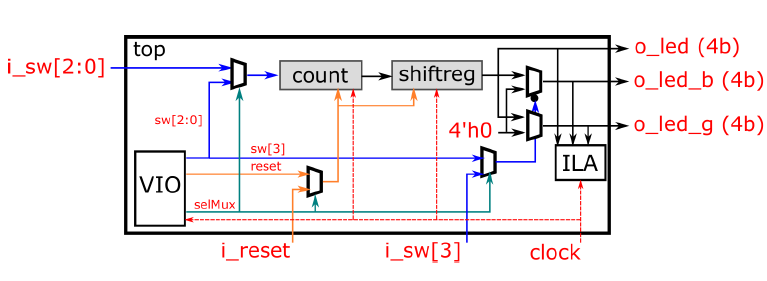
\includegraphics[width=0.9\textwidth]{imagenes_lab01/diagrama_vio_ila.png}
    \caption{Diagrama de implementación del VIO e ILA.}
    \label{fig:diagrama_vio_ila}
\end{figure}

\subsubsection{Verificación por Hardware}
Mediante el protocolo SSH (Secure Shell) se realizó la conexión a la FPGA de forma remota. Esto utilizando la siguiente línea de código desde una terminal.
\begin{terminal}
    ssh -L 3121:172.16.0.231:3121 user@181.231.212.3 -p 2222
\end{terminal}
Con este comando la PC se conecta directamente al servidor de la fundación y activa el puerto 3121, siendo este el puerto que utiliza Vivado por defecto en el Hardware Manager.
Una vez dentro, se simuló el comportamiento y se visualizó la salida mediante el Logic Analyzer.

Teniendo en cuenta que el cambio de valor de la salida \textbf{o\_led}, se muestran a continuación cada uno de los valores posibles en el analizador.

\begin{figure}[H]
    \centering
    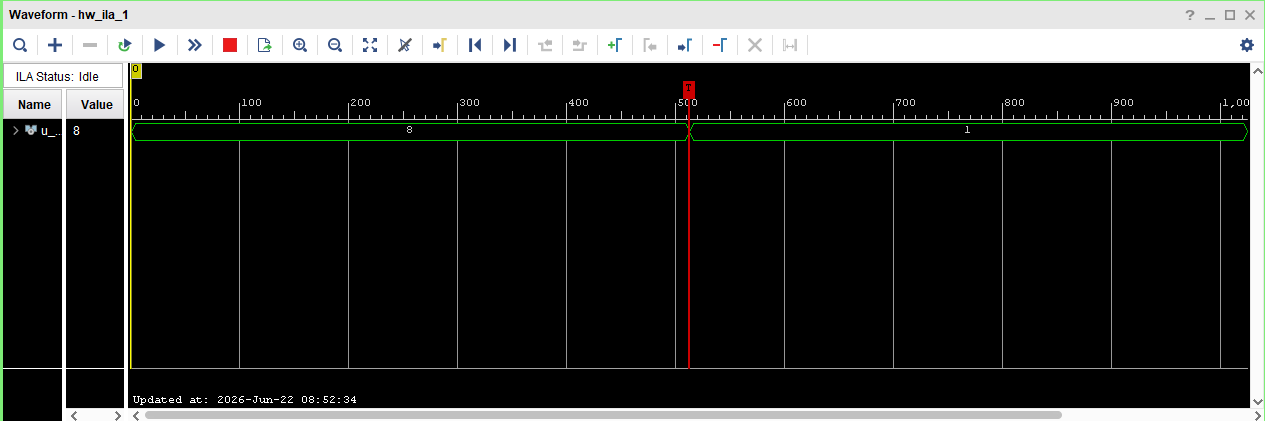
\includegraphics[width=0.9\textwidth]{imagenes_lab01/ila16_r3.png}
    \caption{Waveform de R3 en ILA.}
    \label{fig:ila16_r3}
\end{figure}

Como para el límite superior R3 del contador visto en la figura \autoref{fig:ila16_r3} la cantidad de cambios visibles se reduce, lo que se plantea es cambiar el límite
a un valor menor para verificar el funcionamiento. Según esto, se tienen las siguientes capturas.
\begin{figure}[H]
    \centering
    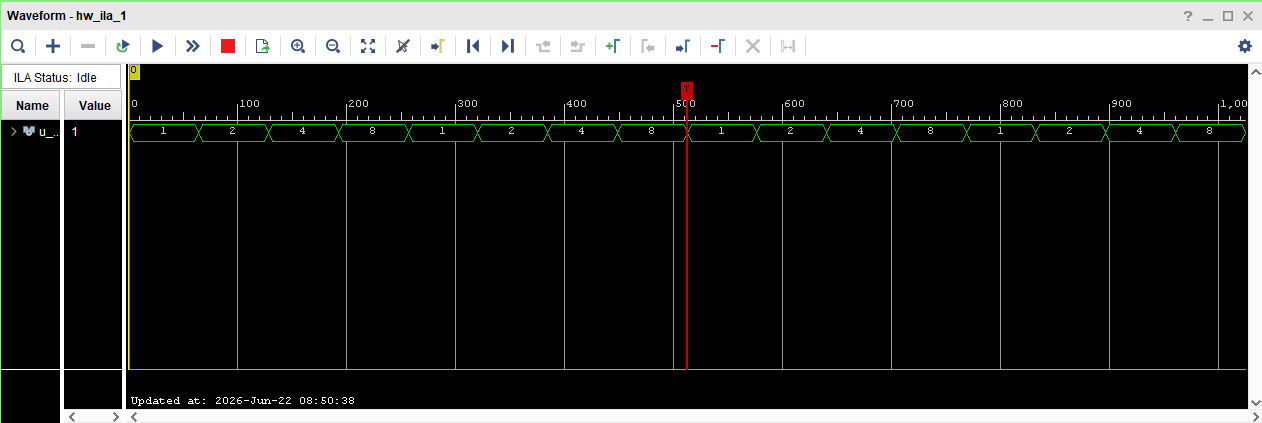
\includegraphics[width=0.9\textwidth]{imagenes_lab01/ila16_r0.png}
    \caption{Waveform de R0 en ILA.}
    \label{fig:ila2_4}
\end{figure}

\begin{figure}[H]
    \centering
    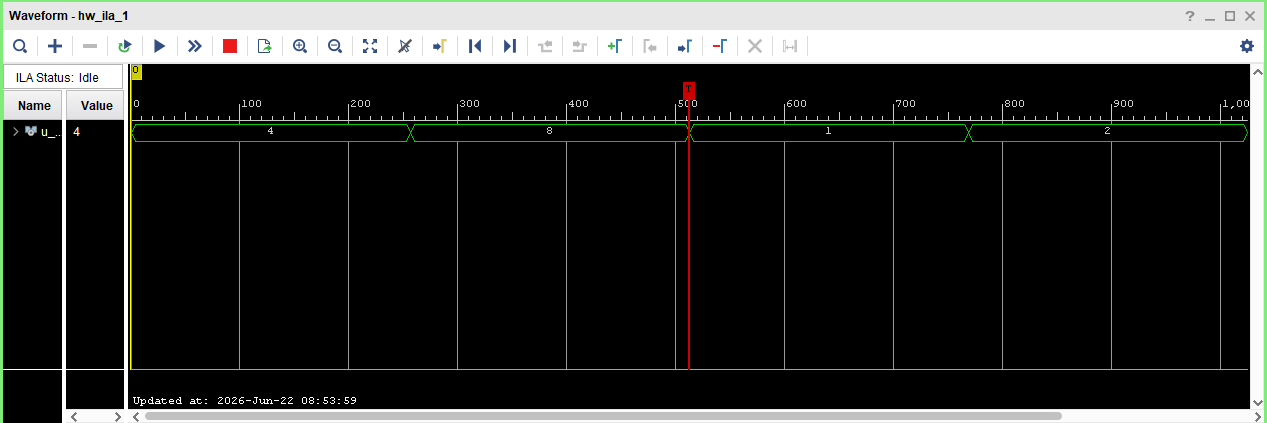
\includegraphics[width=0.9\textwidth]{imagenes_lab01/ila16_r2.png}
    \caption{Waveform de R2 en ILA.}
    \label{fig:ila4_8}
\end{figure}
Utilizando el límite superior \textbf{R2} para una cantidad de bits de contador de 16, se puede ver perfectamente el funcionamiento del sistema.

\newpage
\section{Conclusión}

Dadas las capturas, se concluye que la verificación en FPGA remota fue exitoso, debido que el comportamiento
de la salida es comparable con el funcionamiento del Testbench realizado.

El principal problema presentado en el proceso de prueba se dió en la 
\textbf{Verificación por Hardware}, donde
se tuvo que buscar el valor de bits correcto para el contador, dado que al utilizar un valor muy alto, aumentaba en gran medida
la resolución y no permite ver los cambios de estado correctamente. Se optó por utilizar 16b para este valor.
\end{document}